%%%%%% Run at command line, run
%%%%%% xelatex grad-sample.tex 
%%%%%% for a few times to generate the output pdf file
\documentclass[12pt,oneside,openright,a4paper]{cpe-english-project}

\usepackage{polyglossia}
\setdefaultlanguage{english}
\setotherlanguage{thai}
\newfontfamily\thaifont[Script=Thai,Scale=1.23]{TH Sarabun New}
\defaultfontfeatures{Mapping=tex-text,Scale=1.0,LetterSpace=0.0}
\setmainfont[Scale=1.0,LetterSpace=0,WordSpace=1.0,FakeStretch=1.0]{Times New Roman}

% Custom setting
\setlength{\parskip}{1em} % Set paragraph margin
% Set nested numuric list
\renewcommand{\labelenumii}{\theenumii}
\renewcommand{\theenumii}{\theenumi.\arabic{enumii}.}
\renewcommand{\labelenumiii}{\theenumiii}
\renewcommand{\theenumiii}{\theenumii.\arabic{enumiii}.}
% End set nested numuric list

%\setmathfont(Digits)[Scale=1.0,LetterSpace=0,FakeStretch=1.0]{Times New Roman}


%%%%%%%%%%%%%%%%%%%%%%%%%%%%%%%%%%%%%%%%%%%%%%%%%%%%%%%%%%%%%%%%%%%
% Customize below to suit your needs 
% The ones that are optional can be left blank. 
%%%%%%%%%%%%%%%%%%%%%%%%%%%%%%%%%%%%%%%%%%%%%%%%%%%%%%%%%%%%%%%%%%%
% First line of title
\def\disstitleone{PROJECT NO. 72}   
% Second line of title
\def\disstitletwo{A RESTAURANT RECOMMENDATION SYSTEM FOR INDIVIDUALS AND GROUPS}   
% Your first name and lastname
\def\dissauthor{MR. CHANCHANA WICHA}   % 1st member
\def\dissauthortwo{MS. IRIN YOOKTAJARONG}   % 2nd member (optional)
\def\dissauthorthree{}


% The degree that you're persuing..
\def\dissdegree{Bachelor of Engineering} % Name of the degree
\def\dissdegreeabrev{B.Eng} % Abbreviation of the degree
\def\dissyear{2020}                   % Year of submission
\def\thaidissyear{2563}               % Year of submission (B.E.)

%%%%%%%%%%%%%%%%%%%%%%%%%%%%%%%%%%%%%%%%%%%%
% Your project and independent study committee..
%%%%%%%%%%%%%%%%%%%%%%%%%%%%%%%%%%%%%%%%%%%%
\def\dissadvisor{Dr. Unchalisa Taetragool, Ph.D.}  % Advisor
%%% Leave it empty if you have no Co-advisor
\def\disscoadvisor{}  % Co-advisor
\def\disscommitteetwo{Asst.Prof.Dr. Rajchawit Sarochawikasit, Ph.D.}  % 3rd committee member (optional)
\def\disscommitteethree{Dr. Sally E. Goldin, Ph.D.}   % 4th committee member (optional) 
\def\disscommitteefour{Asst.Prof.Mr. Sanan Srakaew, B.Eng.}    % 5th committee member (optional) 

\def\worktype{Project} %%  Project or Independent study
\def\disscredit{3}   %% 3 credits or 6 credits


\def\fieldofstudy{Computer Engineering} 
\def\department{Computer Engineering} 
\def\faculty{Engineering}

\def\thaifieldofstudy{วิศวกรรมคอมพิวเตอร์} 
\def\thaidepartment{วิศวกรรมคอมพิวเตอร์} 
\def\thaifaculty{วิศวกรรมศาสตร์}
 
\def\appendixnames{Appendix} %%% Appendices or Appendix

\def\thaiworktype{ปริญญานิพนธ์} %  Project or research project % 
\def\thaidisstitleone{หัวข้อปริญญานิพนธ์บรรทัดแรก}
\def\thaidisstitletwo{หัวข้อปริญญานิพนธ์บรรทัดสอง}
\def\thaidissauthor{นายชาญชนะ วิชา}
\def\thaidissauthortwo{นางสาวไอริณ ยุกตจรงค์} %Optional
\def\thaidissauthorthree{} %Optional

\def\thaidissadvisor{ดร. อัญชลิสา แต้ตระกูล}
%% Leave this empty if you have no co-advisor
\def\thaidisscoadvisor{} %Optional
\def\thaidissdegree{วิศวกรรมศาสตรบัณฑิต}

% Change the line spacing here...
\linespread{1.15}

%%%%%%%%%%%%%%%%%%%%%%%%%%%%%%%%%%%%%%%%%%%%%%%%%%%%%%%%%%%%%%%%
% End of personal customization.  Do not modify from this part 
% to \begin{document} unless you know what you are doing...
%%%%%%%%%%%%%%%%%%%%%%%%%%%%%%%%%%%%%%%%%%%%%%%%%%%%%%%%%%%%%%%%


%%%%%%%%%%%% Dissertation style %%%%%%%%%%%
%\linespread{1.6} % Double-spaced  
%%\oddsidemargin    0.5in
%%\evensidemargin   0.5in
%%%%%%%%%%%%%%%%%%%%%%%%%%%%%%%%%%%%%%%%%%%
%\renewcommand{\subfigtopskip}{10pt}
%\renewcommand{\subfigbottomskip}{-5pt} 
%\renewcommand{\subfigcapskip}{-6pt} %vertical space between caption
%                                    %and figure.
%\renewcommand{\subfigcapmargin}{0pt}

\renewcommand{\topfraction}{0.85}
\renewcommand{\textfraction}{0.1}

\newtheorem{theorem}{Theorem}
\newtheorem{lemma}{Lemma}
\newtheorem{corollary}{Corollary}

\def\QED{\mbox{\rule[0pt]{1.5ex}{1.5ex}}}
\def\proof{\noindent\hspace{2em}{\itshape Proof: }}
\def\endproof{\hspace*{\fill}~\QED\par\endtrivlist\unskip}
%\newenvironment{proof}{{\sc Proof:}}{~\hfill \blacksquare}
%% The hyperref package redefines the \appendix. This one 
%% is from the dissertation.cls
%\def\appendix#1{\iffirstappendix \appendixcover \firstappendixfalse \fi \chapter{#1}}
%\renewcommand{\arraystretch}{0.8}
%%%%%%%%%%%%%%%%%%%%%%%%%%%%%%%%%%%%%%%%%%%%%%%%%%%%%%%%%%%%%%%%
%%%%%%%%%%%%%%%%%%%%%%%%%%%%%%%%%%%%%%%%%%%%%%%%%%%%%%%%%%%%%%%%


\begin{document}
\pdfstringdefDisableCommands{%
\let\MakeUppercase\relax
}
\begin{center}
  
\includegraphics[width=2.8cm]{logo02.jpg}
\end{center}
\vspace*{-1cm}

\maketitlepage
\makesignaturepage 

%%%%%%%%%%%%%%%%%%%%%%%%%%%%%%%%%%%%%%%%%%%%%%%%%%%%%%%%%%%%%%
%%%%%%%%%%%%%%%%%%%%%% English abstract %%%%%%%%%%%%%%%%%%%%%%%
%%%%%%%%%%%%%%%%%%%%%%%%%%%%%%%%%%%%%%%%%%%%%%%%%%%%%%%%%%%%%%
\abstract

In recent years, recommendation systems are widely used for movies, music, or products in order to reduce the time and effort of the users’ searching and increase users’ experience. However, restaurant recommendation systems are still very few in this industry and the existing recommenders in Thailand are just randomization applications and the majority of recommender systems are designed for individual users. In contrast, since this activity or event usually occurs in a group of people, not just individually, which each person can have the same or different behaviors, preferences, and interests. Therefore, group decisions often differ from individual decisions. As a result, each decision is often taken longer than one person, and sometimes conclusions are not able to be drawn or it may cause conflicts within the group.

According to the mentioned problems, we were motivated to develop this project, A Restaurant Recommendation System for Individuals and Groups, to better assist in group decision making. Our project is a web application that recommends restaurants in the Bangkok area to users based on their behaviors, preferences, and interests of both individuals and groups eating. The genetic algorithm is applied for generating suitable recommended restaurants for users. Therefore, this project aims to reduce time-wasting of decision making for both individuals and groups and increase the users’ experience and satisfaction when using our recommendation system.


\begin{flushleft}
\begin{tabular*}{\textwidth}{@{}lp{0.8\textwidth}}
\textbf{Keywords}: & Genetic Algorithm / Optimization Problem / Decision Making Process / Group Recommendation Systems / Web Application / Restaurants
\end{tabular*}
\end{flushleft}
\endabstract

%%%%%%%%%%%%%%%%%%%%%%%%%%%%%%%%%%%%%%%%%%%%%%%%%%%%%%%%%%%%%%
%%%%%%%%%% Thai abstract here %%%%%%%%%%%%%%%%%%%%%%%%%%%%%%%%%
%%%%%%%%%%%%%%%%%%%%%%%%%%%%%%%%%%%%%%%%%%%%%%%%%%%%%%%%%%%%%%
{
\XeTeXlinebreaklocale "th_TH"	
\thaifont
\thaiabstract

ในช่วงไม่กี่ปีที่ผ่านมาได้มีการใช้ระบบแนะนำ (Recommendation System) อย่างแพร่หลายไม่ว่าจะเป็นภาพยนตร์ เพลง หรือระบบแนะนำผลิตภัณฑ์ต่าง ๆ เพื่อลดระยะเวลาและความยุ่งยากในการค้นหาของผู้ใช้รวมถึงเพิ่มประสบการณ์ของผู้ใช้อย่างไรก็ตามระบบแนะนำร้านอาหารยังมีน้อยมากในวงการระบบคำแนะนำนอกจากนั้นระบบแนะนำร้านอาหารที่มีอยู่ในประเทศไทยเป็นเพียงแอปพลิเคชันแบบสุ่มและส่วนใหญ่ออกแบบมาสำหรับผู้ใช้แต่ละรายเท่านั้น ซึ่งในความเป็นจริงแล้วการรับประทานอาหารมักเกิดขึ้นเป็นกลุ่มตั้งแต่ 2 คนขึ้นไปไม่ได้เป็นรายบุคคลเพียงอย่างเดียว ซึ่งแต่ละคนในกลุ่มนั้นมีพฤติกรรม ความชอบและความสนใจที่อาจจะเหมือนหรือแตกต่างกันดังนั้นการตัดสินใจของกลุ่มมักแตกต่างจากการตัดสินใจของแต่ละบุคคล ด้วยเหตุนี้การตัดสินใจในแต่ละครั้ง มักใช้เวลานานกว่าการตัดสินใจด้วยคน ๆ เดียว และในบางครั้งการตัดสินใจนั้นอาจจะไม่สามารถหาข้อสรุปได้ หรืออาจทําให้เกิดความขัดแย้งขึ้นภายในกลุ่ม

ด้วยเหตุนี้เอง ทางผู้พัฒนาจึงมีความตั้งใจที่จะพัฒนาเว็บแอปพลิเคชันสำหรับแนะนำร้านอาหารที่อยู่ในพื้นที่จังหวัดกรุงเทพมหานครสำหรับรายบุคคลและรายกลุ่มขึ้น เพื่อเป็นตัวช่วยในการตัดสินใจทั้งแบบเดี่ยวและกลุ่มได้ดีมากยิ่งขึ้น โดยระบบแนะนําร้านอาหารจะอ้างอิงจากข้อมูลของผู้ใช้งาน ไม่ว่าจะเป็นพฤติกรรม ความสนใจ หรือความชอบ ทั้งแบบเดี่ยวและกลุ่ม ด้วยขั้นตอนวิธีเชิงพันธุกรรม (Genetic Algorithm) ในการหาค่าเหมาะสมที่สุดเชิงคณิตศาสตร์ (Mathematical Optimization) สุดท้ายนี้ผู้พัฒนามีความมุ่งหวังว่าระบบแนะนําร้านอาหารรายบุคคลและรายกลุ่มในโครงงานนี้จะช่วยลดเวลาที่เสียไปในการตัดสินใจและเพิ่มความพึงพอใจของผู้ใช้งานต่อร้านอาหารที่ระบบได้ทำการแนะนำ


\begin{flushleft}
\begin{tabular*}{\textwidth}{@{}lp{0.8\textwidth}}
 & \\

\textbf{คำสำคัญ}: & ขั้นตอนวิธีเชิงพันธุกรรม / การหาค่าเหมาะสมที่สุดเชิงคณิตศาสตร์ / กระบวนการการตัดสินใจ / ระบบแนะนำรายกลุ่ม / เว็บแอปพลิเคชัน / ร้านอาหาร
\end{tabular*}
\end{flushleft}
\endabstract
}

%%%%%%%%%%%%%%%%%%%%%%%%%%%%%%%%%%%%%%%%%%%%%%%%%%%%%%%%%%%%
%%%%%%%%%%%%%%%%%%%%%%% Acknowledgments %%%%%%%%%%%%%%%%%%%%
%%%%%%%%%%%%%%%%%%%%%%%%%%%%%%%%%%%%%%%%%%%%%%%%%%%%%%%%%%%%
\preface
Throughout the writing of this project we have received a great deal of support and assistance.

We would like to express my very great appreciation to Dr. Unchalisa Taetragool for her valuable and constructive suggestions during the planning and development of this project work. Her willingness to give his time so generously has been very much appreciated.

We would also like to express our very great appreciation to our committees, Asst.Prof.Dr. Rajchawit Sarochawikasit, Dr. Sally E. Goldin and Asst.Prof.Mr. Sanan Srakaew, for their valuable guidelines and suggestions throughout our studies.

We also appreciate the Department of Computer Engineering for providing the laboratory and resources for the implementation of this project.

In addition, we would like to thank our parents for their wise counsel and sympathetic ear. You are always there for us. We could not have completed this project without the support of my friends who provided the feedback and suggestions throughout the development process. Finally, we would like to thank Avril Lavigne for entertaining us while we were writing this report.


%%%%%%%%%%%%%%%%%%%%%%%%%%%%%%%%%%%%%%%%%%%%%%%%%%%%%%%%%%%%%
%%%%%%%%%%%%%%%% ToC, List of figures/tables %%%%%%%%%%%%%%%%
%%%%%%%%%%%%%%%%%%%%%%%%%%%%%%%%%%%%%%%%%%%%%%%%%%%%%%%%%%%%%
% The three commands below automatically generate the table 
% of content, list of tables and list of figures
\tableofcontents                    
\listoftables
\listoffigures                      

%%%%%%%%%%%%%%%%%%%%%%%%%%%%%%%%%%%%%%%%%%%%%%%%%%%%%%%%%%%%%%
%%%%%%%%%%%%%%%%%%%%% List of symbols page %%%%%%%%%%%%%%%%%%%
%%%%%%%%%%%%%%%%%%%%%%%%%%%%%%%%%%%%%%%%%%%%%%%%%%%%%%%%%%%%%%
% You have to add this manually..
\listofsymbols
\begin{flushleft}
\begin{tabular}{@{}p{0.07\textwidth}p{0.7\textwidth}p{0.1\textwidth}}
\textbf{SYMBOL}  & & \textbf{UNIT} \\[0.2cm]
$\alpha$ & Test variable\hfill & m$^2$ \\
$\lambda$ & Interarival rate\hfill &  jobs/second\\
$\mu$ & Service rate\hfill & jobs/second\\
\end{tabular}
\end{flushleft}
%%%%%%%%%%%%%%%%%%%%%%%%%%%%%%%%%%%%%%%%%%%%%%%%%%%%%%%%%%%%%%
%%%%%%%%%%%%%%%%%%%%% List of vocabs & terms %%%%%%%%%%%%%%%%%
%%%%%%%%%%%%%%%%%%%%%%%%%%%%%%%%%%%%%%%%%%%%%%%%%%%%%%%%%%%%%%
% You also have to add this manually..
\listofvocab
\begin{flushleft}
\begin{tabular}{@{}p{1in}@{=\extracolsep{0.5in}}l}
ABC & Adaptive Bandwidth Control \\
MANET & Mobile Ad Hoc Network 
\end{tabular}
\end{flushleft}

%\setlength{\parskip}{1.2mm}

%%%%%%%%%%%%%%%%%%%%%%%%%%%%%%%%%%%%%%%%%%%%%%%%%%%%%%%%%%%%%%%
%%%%%%%%%%%%%%%%%%%%%%%% Main body %%%%%%%%%%%%%%%%%%%%%%%%%%%%
%%%%%%%%%%%%%%%%%%%%%%%%%%%%%%%%%%%%%%%%%%%%%%%%%%%%%%%%%%%%%%%


\chapter{Introduction}

\section{Keywords} 

Genetic Algorithm, Optimization Problem, Decision Making Process, Group Recommendation Systems, Web Application, Restaurants

\section{Problem Statement, Motivation, and Potential Benefits} 

“Kin-Rai-Dee? (Where are we going to eat?)” is the most common phrase we ask ourselves and others almost every day. We also believe that many people will as well ask this simple question regularly around mealtimes whether they are going to eat alone or with their group. To decide what and where to eat can take more time than necessary which can lead to frustration and sometimes, in the end, the decision cannot be made.

From the problems online survey, it revealed that 62\% of the respondents, 93 out of 148, felt restaurant selection in each meal is their main problem which up to 65.5 \% faced the pain about restaurant selection in a group by occurring frequently in a group of friends. The major issue comes from a variety of factors and conditions which lead to the inability to decide. From further inquiries about how they solved the problem, we found that very few people will find a restaurant that matches the conditions of their group. They usually select the restaurant according to the majority which cannot serve everyone’s satisfaction. Some of them use the recommendation application to be their alternative way to decide. Moreover, in the worst case, they just eat separately. 

Even though various applications can suggest food to users, almost all of them just randomize the suggestions without any logic. Moreover, many of them suggest only food, not a restaurant. Based on our research, some applications that can suggest a restaurant based on their users’ preference still cannot support a suggestion for a group.

In this project, we will implement a web application that can solve the mentioned problems and improve the existing solutions. Our application will recommend a restaurant based on individual or group preferences, behaviors, and customizations. We hope that the application will be able to reduce time-wasting in choosing restaurants and give us no more frustration.

\section{Project Type} 
Potential Commercial Product

\section{Proposed Method} 
\subsection{Approach} 
From the problem statement above, we will develop a web application that suggests a restaurant that matches customer profiles. We will provide a diversity of restaurants in Bangkok from an external source and their general information that facilitate their restaurant consideration. Also, we will suggest a restaurant that matches multiple preferences (multiple users) by multi-objective optimization algorithms.

\subsubsection{Literature Review and Survey} 
Explore existing works and knowledge related to our project e.g. recommendation system, multi-objective optimization algorithms, machine learning model, software engineering for web application development, etc. Moreover, we survey and construct a customer journey.

\subsubsection{Data Collection} 
Gather a restaurant profile from an external source which is the restaurant's Facebook pages. and user profile from our data collection tool.

\subsubsection{Data Preparation} 
A preprocessing method includes cleaning, selecting, normalizing, transforming, etc. to be a training set.

\subsubsection{Construct the Model} 
Design and construct a model and train with prepared data, model evaluation, and hyperparameter tuning. This model will be integrated with our backend service.

\subsubsection{Design User Interface} 
Design an user interface for our web application. This design process includes prototype implementation and prototype testing which can improve the user experience.

\subsubsection{Build a Web Application} 
Implement a web application from our design. This implementation includes frontend and backend development.

\subsubsection{Validation} 
Validate our completed web application which integrated our model. This process includes feedback gathering from users, feedback evaluation, model performance evaluation, and application performance monitoring.


\subsection{Objectives} 
\begin{itemize}
\item  To collect and analyze the customer behavioral data.
\item  To implement an analytical model that can suggest the right restaurant to individuals or a group of people based on their preferences, profiles, and behaviors.
\item  To implement a web application that allows users and groups of users to input their preferences and obtain the recommended restaurants.
\item To reduce time-wasting on a restaurant consideration. 
\end{itemize}

\subsection{Scope} 
\begin{itemize}
\item Our web application supports modern web browsers such as Google Chrome, Safari, Firefox.
\item Our web application focuses on the person or group of people who eat in the restaurant (not focus on delivery).
\item Internet access is required in order to use our application.
\item Restaurants in our database obtained from an external source are only restaurants in Bangkok.
\end{itemize}


\section{Original Engineering Content} 
In this project, we will develop the following software, dataset, and algorithm:

\subsection{Web Application} 
A web application for users that suggests the right restaurant to the right people based on individual preferences and group preferences. This application also collects customer behavior data as well as feedback from users.

\subsection{Customer Behavior Dataset} 
Customer behavior data will be collected throughout semesters by both our data collection tool which will be used before our final product and our web application. The data include the restaurant that users choose to go with time series and their demographic information.

\subsection{Group Recommendation Algorithm} 
Our system will recommend restaurants to individuals or groups by using our recommendation algorithm which includes machine learning and multi-objective optimization algorithms.


\section{Task Breakdown and Draft Schedule}
\subsection{Semester 1}
\begin{enumerate}
  \item Requirement Gathering
  \begin{enumerate}
    \item Kick-off meeting
    \item Brainstorm and analysis
    \item Survey
     \begin{enumerate}
      \item Competitor survey
      \item Paper survey
      \item Target user survey
      \item Market survey
     \end{enumerate}
    \item Survey conclusion
    \item Requirement conclusion
  \end{enumerate}
  \item Create Proposal
  \item Researching
  \begin{enumerate}
   \item Recommendation algorithm researching
   \item Optimization algorithm researching
  \end{enumerate}
  \item Midterm Project Presentation (Slide and video presentation)
  \item Data Collection Phase I
  \begin{enumerate}
   \item Restaurant profile collection from sources
   \item Implement user data gathering tool
   \item User profile collection from tool
  \end{enumerate}
  \item Design
  \begin{enumerate}
   \item UX/UI Design
   	\begin{enumerate}
  	 \item Customer journey
      \item Create wireframe
      \item Test wireframe
      \item UI design
      \item Prototype implementation
      \item Test prototype
     \item Improvement
      \end{enumerate}
     \item Architecture Design
   	\begin{enumerate}
  	 \item System architecture
      \item Database
      \end{enumerate}
  \end{enumerate}
  \item Create Final Report
  \item Final Project Presentation (Slide and video presentation)
\end{enumerate}


\subsection{Semester 2}
\begin{enumerate}
 \item Development
 \begin{enumerate}
  \item Application Development
  \begin{enumerate}
   \item Web application implementation
   \item Testing
   \item Application improvement
  \end{enumerate}
  \item Model Development
  \begin{enumerate}
   \item Model construction and training
   \item Model evaluation
   \item Model improvement
  \end{enumerate}
  \item Integration Testing
  \begin{enumerate}
   \item Testing
   \item Debugging
  \end{enumerate}
  \item User Acceptance Testing
  \begin{enumerate}
   \item User testing
   \item User feedback gathering
   \item Feedback evaluation
   \item System improvement
  \end{enumerate}
  \item Create Report and Presentation
  \item Production Deployment
  \begin{enumerate}
   \item Backend deployment
   \item Frontend deployment
   \item Production testing
  \end{enumerate}
 \end{enumerate}
\end{enumerate}

\begin{figure}[!h]\centering
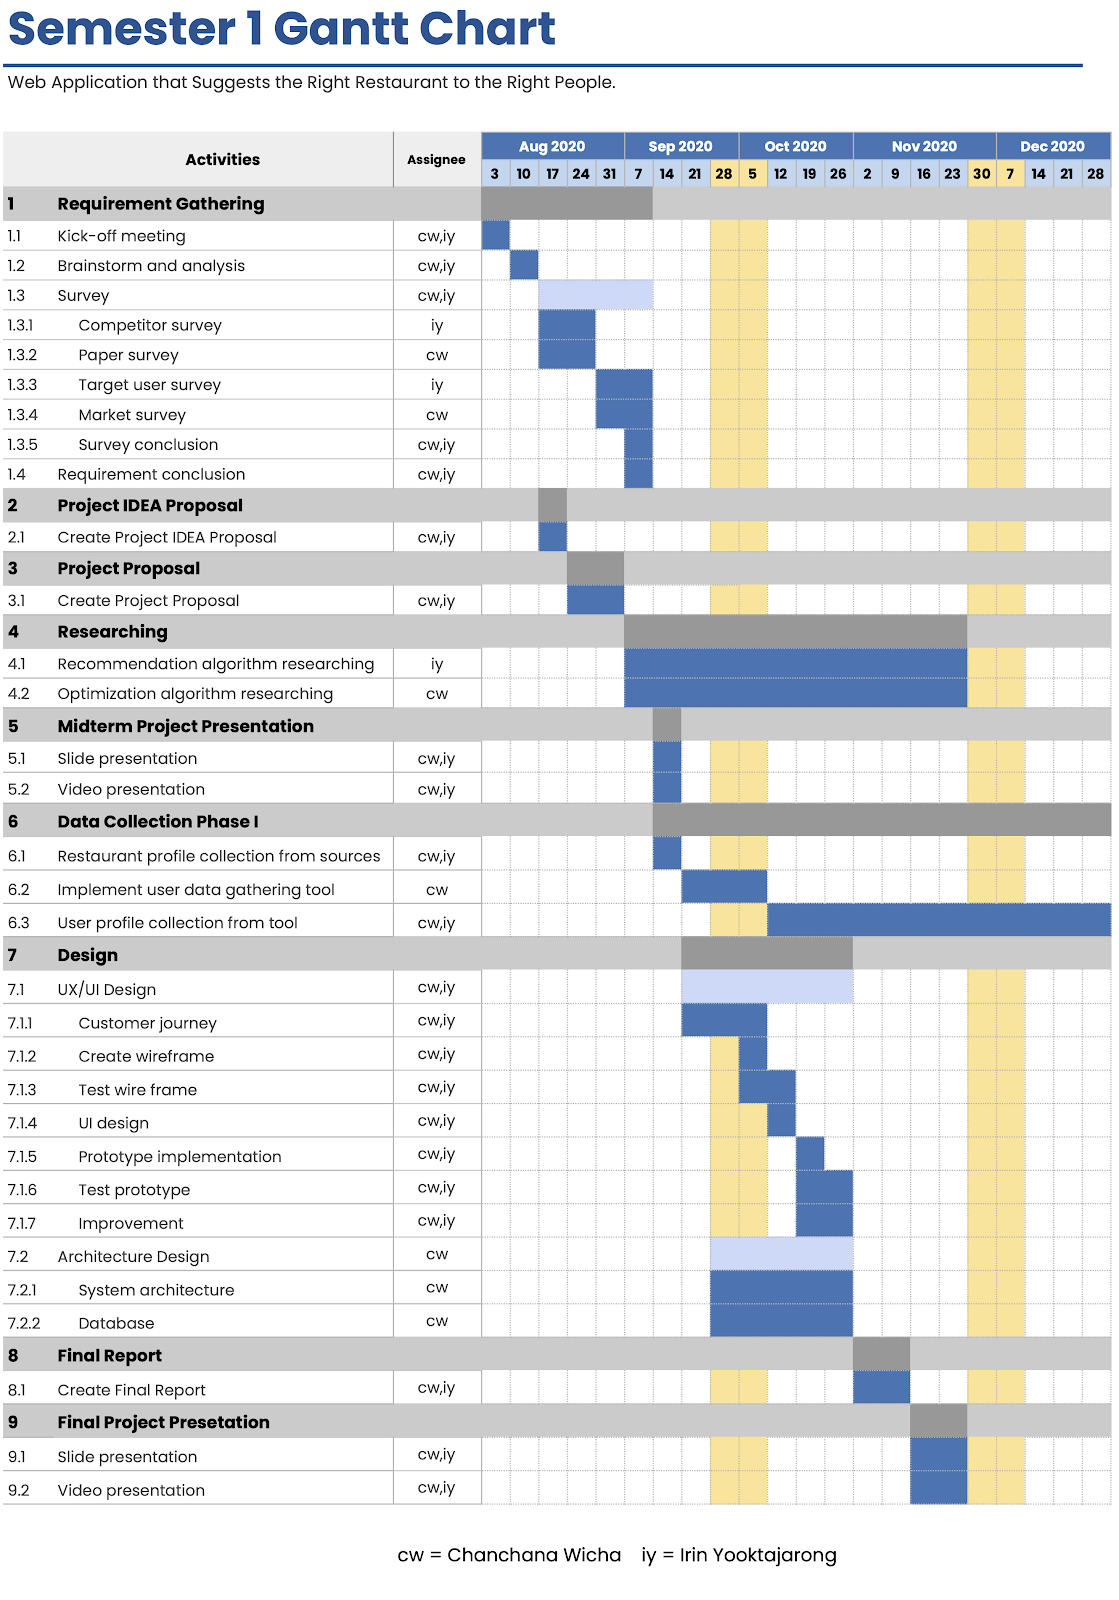
\includegraphics[width=440pt]{./images/1gantt1.png}
\caption{Gantt Chart for the First Semester}\label{fig:1_1}
\end{figure}

\begin{figure}[!h]\centering
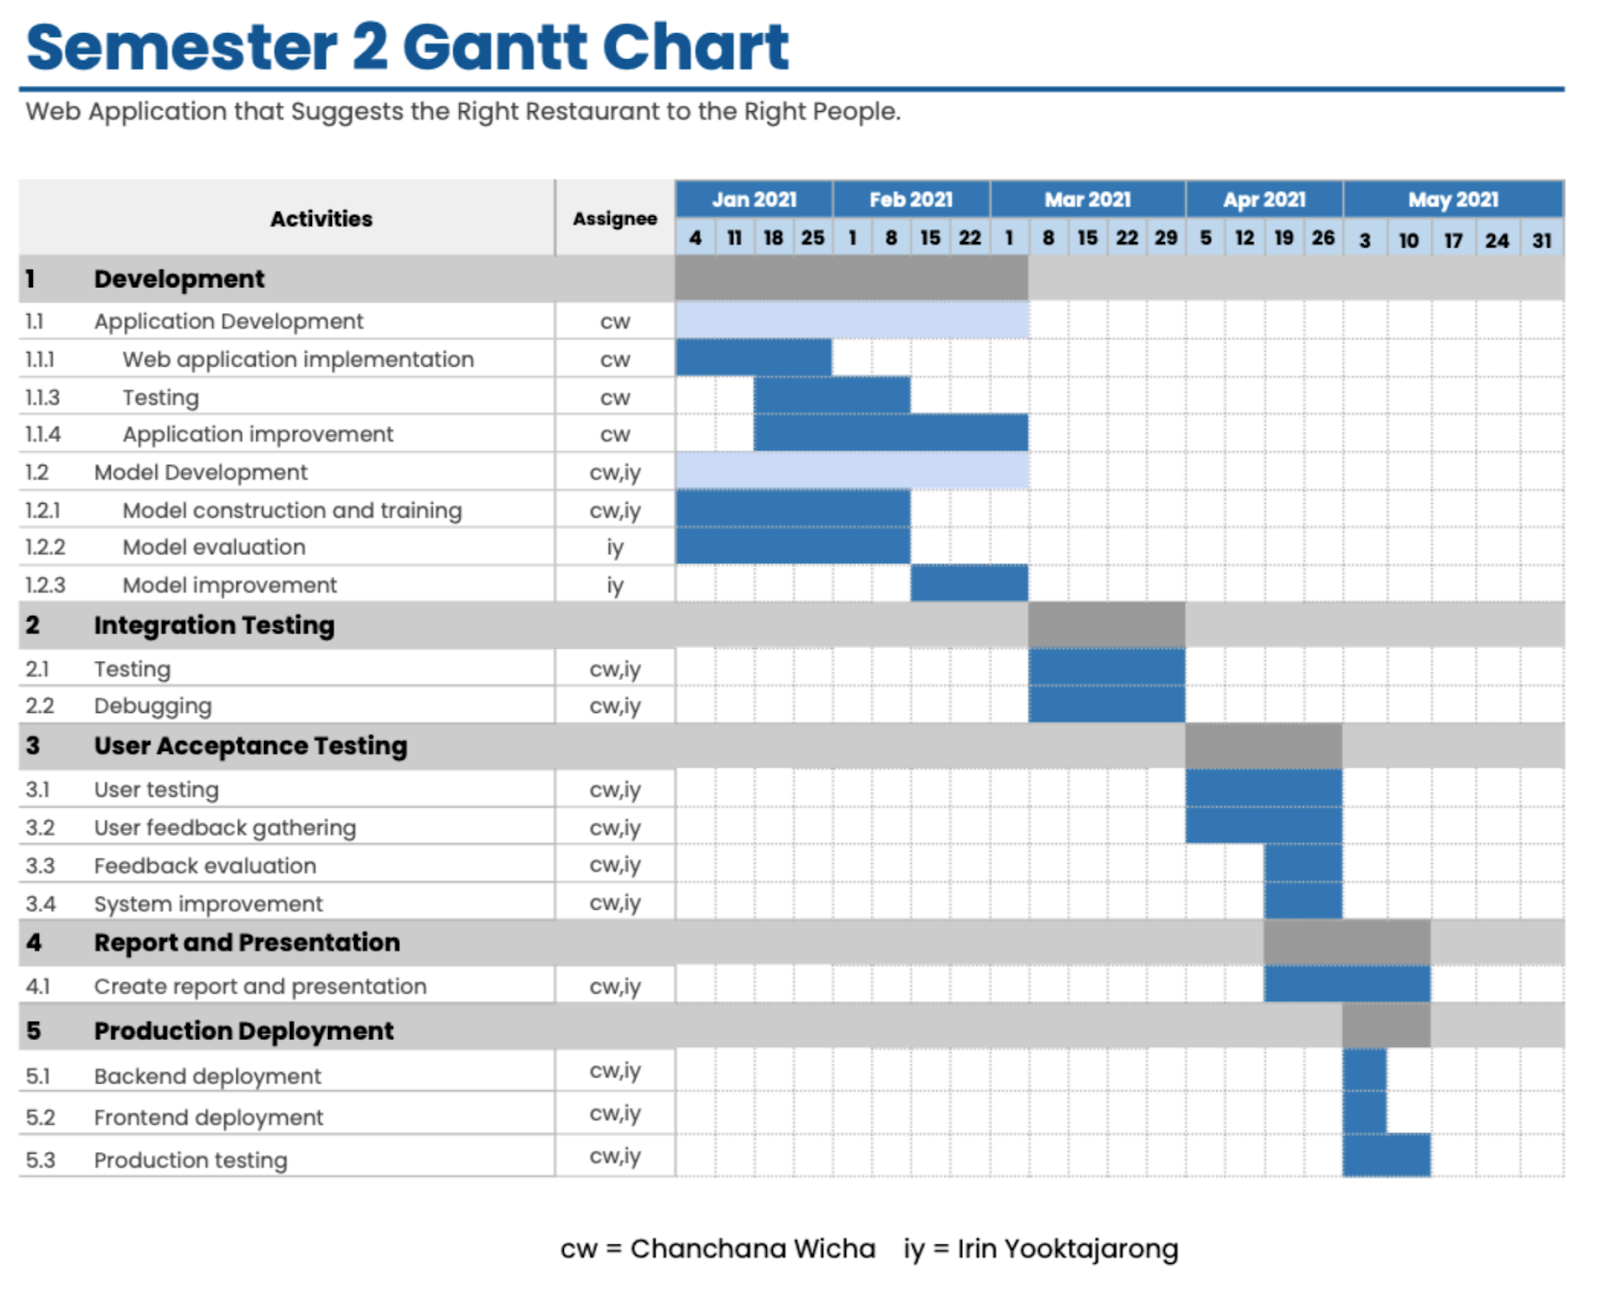
\includegraphics[width=440pt]{./images/1gantt2.png}
\caption{Gantt Chart for the Second Semester}\label{fig:1_2}
\end{figure}

\newpage

\section{Deliverables for Term 1} 
\begin{itemize}
\item Requirement Specification
\item Survey Result
\item Data Collection Tool
\item Dataset (Customer Behavior and Restaurant Information)
\item Customer Journey
\item Prototype (Web Application)
\item Database Schema
\item System Architecture and Class Diagram
\item Suggestion Algorithm and Model
\end{itemize}

\section{Deliverables for Term 2} 
\begin{itemize}
\item Web Application (Frontend and Backend)
\item Recommendation System both Individuals and Groups
\item Feedback from Users
\item Application Performance Evaluation
\item Model Performance Evaluation
\end{itemize}


\end{document}

%%%%%%%%%%%%%%%%%%%%%%%%%%%%%%%%%%%%%%%%%%%%%%%%%%%%%%%%%%%%
%%%%%%%%%%%%%%  Literature Review %%%%%%%%%%%%%%%%%%%%%%%%%%
%%%%%%%%%%%%%%%%%%%%%%%%%%%%%%%%%%%%%%%%%%%%%%%%%%%%%%%%%%%%
\chapter{Background Theory and Related Work}

\url{http://www.cpe.kmutt.ac.th}
Explain theory, algorithms, protocols, or existing research works and tools related to your work. \cite{bworld}

\section{Recommender Systems}

\begin{table}[!h]
\caption{test table method1}\label{tbl:method1}
\begin{tabular}{c|c|l|rr} \hline\hline
Center & Center & left aligned & Right & Right aligned \\ \hline\hline
Center & Center & left aligned & Right & Right aligned \\ \hline
Center & Center & left aligned & Right & Right aligned \\ 
Center & Center & left aligned & Right & Right aligned \\ \hline
Center & Center & left aligned & Right & Right aligned \\ \hline\hline
\end{tabular}
\end{table}


\section{Text Processing Algorithms}
\subsection{Algorithm I}

% Can define this in the preamble..
You can place the figure and refer to it as Figure~\ref{fig:model2}.
The figure and table numbering will be run and updated automatically when you add/remove tables/figures from the document.

\begin{figure}[!h]\centering
\setlength{\fboxrule}{0.2mm} % can define this in the preamble
\setlength{\fboxsep}{1cm}
\fbox{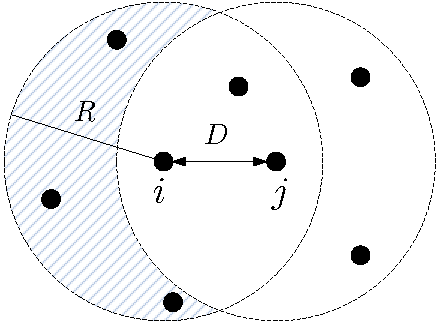
\includegraphics[width=5cm]{./model2.pdf}}
\caption{The network model}\label{fig:model2}
\end{figure}

 
\subsection{Algorithm II}
Add more subsections as you want.

\subsubsection{Algorithm SUB}
Add more subsections as you want.


\section{Development Tools}

%%%%%%%%%%%%%%%%%%%%%%%%%%%%%%%%%%%%%%%%%%%%%%%%%%%%%55
%%%%%%%%%%%%%%%%%%%%%%%%%%%%%%%%%%%%%%%%%%%%%%%%%%%%%
%%%%%%%%%%%%%%%%%%%%%%%%%%%%%%%%%%%%%%%%%%%%%%%%%%%%%
\chapter{Proposed Work}

Explain the design (how you plan to implement your work) of your project. Adjust the section titles below to suit the types of your work. Detailed physical design like circuits and source codes should be placed in the appendix.

\section{System Architecture}

\begin{table}[!h]
\centering
\caption{test table x1}\label{tbl:symbols}
\begin{tabular}{@{}p{0.07\textwidth}|p{0.7\textwidth}p{0.1\textwidth}}\hline
\multicolumn{2}{l}{\textbf{SYMBOL}}  & \textbf{UNIT} \\ \hline 
$\alpha$ & Test variable\hfill & m$^2$ \\
$\lambda$ & Interarrival rate\hfill &  jobs/second\\
$\mu$ & Service rate\hfill & jobs/second \\ \hline
\end{tabular}
%\begin{tabular}{c|c} \hline
% $\alpha$ & $\beta$ \\ \hline
% $\delta$ & $\mu$ \\ \hline
%\end{tabular}
\end{table}

\section{System Specifications and Requirements}

\section{Hardware Module 1}
\subsection{Component 1}
\subsection{Logical Circuit Diagram}

\section{Hardware Module 2}
\subsection{Component 1}
\subsection{Component 2}

\section{Path Finding Algorithm}

\section{Database Design}

\section{GUI Design}



%%%%%%%%%%%%%%%%%%%%%%%%%%%%%%%%%%%%%%%%%%%%%%%%%%%%%%%%%%%%%%
%%%%%%%%%%%%%%%%%%%% Experiments %%%%%%%%%%%%%%%%%%%%%%%%%%%%%
%%%%%%%%%%%%%%%%%%%%%%%%%%%%%%%%%%%%%%%%%%%%%%%%%%%%%%%%%%%%%%%
\chapter{Implementation Results}

You can title this chapter as \textbf{Preliminary Results} or \textbf{Work Progress} for the progress reports. Present implementation or experimental results here and discuss them.

%%%%%%%%%%%%%%%%%%%%%%%%%%%%%%%%%%%%%%%%%%%%%%%%%%%%%%%%%%%%%%%
%%%%%%%%%%%%%%%%%%%% Conclusions %%%%%%%%%%%%%%%%%%%%%%%%%%%%%
%%%%%%%%%%%%%%%%%%%%%%%%%%%%%%%%%%%%%%%%%%%%%%%%%%%%%%%%%%%%%%%
\chapter{Conclusions}

This chapter is optional for proposal and progress reports but 
is required for the final report.

\section{Problems and Solutions}
State your problems and how you fixed them.

\section{Future Works}
What could be done in the future to make your projects better.

%%%%%%%%%%%%%%%%%%%%%%%%%%%%%%%%%%%%%%%%%%%%%%%%%%%%%%%%%%%%%%%
%%%%%%%%%%%%%%%%%%%% Bibliography %%%%%%%%%%%%%%%%%%%%%%%%%%%%%
%%%%%%%%%%%%%%%%%%%%%%%%%%%%%%%%%%%%%%%%%%%%%%%%%%%%%%%%%%%%%%%

%%%% Comment this in your report to show only references you have
%%%% cited. Otherwise, all the references below will be shown.
\nocite{*}
%% Use the kmutt.bst for bibtex bibliography style 
%% You must have cpe.bib and string.bib in your current directory.
%% You may go to file .bbl to manually edit the bib items.
\bibliographystyle{kmutt}
\bibliography{string,cpe}

%%%%%%%%%%%%%%%%%%%%%%%%%%%%%%%%%%%%%%%%%%%%%%%%%%%%%%%%%%%%%%%
%%%%%%%%%%%%%%%%%%%%%%%% Appendix %%%%%%%%%%%%%%%%%%%%%%%%%%%%%
%%%%%%%%%%%%%%%%%%%%%%%%%%%%%%%%%%%%%%%%%%%%%%%%%%%%%%%%%%%%%%%
\appendix{First appendix title}
\noindent{\large\bf Put appropriate topic here} \\

This is where you put hardware circuit diagrams, detailed experimental data in tables or source codes, etc.. \\ \bigskip



This appendix describes two static allocation methods for fGn (or fBm)
traffic. Here, $\lambda$ and $C$ are respectively the traffic arrival
rate and the service rate per dimensionless time step. Their unit are
converted to a physical time unit by multiplying the step size
$\Delta$. For a fBm self-similar traffic source,
Norros~\cite{norros95} provides its EB as
\begin{equation}\label{eq:norros}
  C = \lambda + (\kappa(H)\sqrt{-2\ln\epsilon})^{1/H}a^{1/(2H)}x^{-(1-H)/H}\lambda^{1/(2H)}
\end{equation}
where $\kappa(H) = H^H(1-H)^{(1-H)}$. Simplicity in the calculation is
the attractive feature of (\ref{eq:norros}).

The MVA technique developed in~\cite{kim01} so far provides the most
accurate estimation of the loss probability compared to previous
bandwidth allocation techniques according to simulation results.
Consider a discrete-time queueing system with constant service rate
$C$ and input process $\lambda_n$ with $\mathbb{E}\{\lambda_n\} =
\lambda$ and $\mathrm{Var}\{\lambda_n\} = \sigma^2$.  Define $X_n \equiv
\sum_{k=1}^n \lambda_k - Cn$.  The loss probability due to the MVA
approach is given by
\begin{equation}\label{eq:loss_mva}
  \varepsilon \approx \alpha e^{-m_x/2}
\end{equation}
where
\begin{equation}\label{eq:mx}
m_x = \min_{n \geq 0} \frac{((C-\lambda)n + B)^2}{\mathrm{Var}\{X_n\}} =
\frac{((C-\lambda)n^\ast + B)^2}{\mathrm{Var}\{X_{n^{\ast}}\}}
\end{equation} 
and 
\begin{equation}\label{eq:alpha}
  \alpha =
  \frac{1}{\lambda\sqrt{2\pi\sigma^2}}\exp\left(\frac{(C-\lambda)^2}{2\sigma^2}\right)
  \int_C^\infty (r-C)\exp\left(\frac{(r-\lambda)^2}{2\sigma^2}\right)\, dr
\end{equation}
For a given $\varepsilon$, we numerically solve for $C$ that satisfies
(\ref{eq:loss_mva}). Any search algorithm can be used to do the task.
Here, the bisection method is used.  

Next, we show how $\mathrm{Var}\{X_n\}$ can be determined.  Let
$C_{\lambda}(l)$ be the autocovariance function of $\lambda_n$.  The
MVA technique basically approximates the input process $\lambda_n$
with a Gaussian process, which allows $\mathrm{Var}\{X_n\}$ to be
represented by the autocovariance function.  In particular, the
variance of $X_n$ can be expressed in terms of $C_{\lambda}(l)$ as
\begin{equation}
  \mathrm{Var}\{X_n\} = nC_{\lambda}(0) + 2\sum_{l=1}^{n-1} (n-l)C_{\lambda}(l)
\end{equation} 
Therefore, $C_{\lambda}(l)$ must be known in the MVA technique, either
by assuming specific traffic models or by off-line analysis in case of
traces.  In most practical situations, $C_{\lambda}(l)$ will not be
known in advance, and an on-line measurement algorithm developed
in~\cite{eun01} is required to jointly determine both $n^\ast$ and
$m_x$. For fGn traffic, $\mathrm{Var}\{X_n\}$ is equal to $\sigma^2
n^{2H}$, where $\sigma^2 = \mathrm{Var}\{\lambda_n\}$, and we can find
the $n^\ast$ that minimizes (\ref{eq:mx}) directly. Although $\lambda$
can be easily measured, it is not the case for $\sigma^2$ and $H$.
Consequently, the MVA technique suffers from the need of prior
knowledge traffic parameters.


%%%%%%%%%%%%%%%%%%%%%%%%%%%%%%%%%%%%%%%%%%%%%%%%%%%%%%%%%%
%%%%%%%%%%%%%%% The 2nd appendix %%%%%%%%%%%%%%%%%%%%%%%%%%
%%%%%%%%%%%%%%%%%%%%%%%%%%%%%%%%%%%%%%%%%%%%%%%%%%%%%%%%%%
\appendix{Second appendix title}
\noindent{\large\bf Put appropriate topic here} \\

Next, we show how $\mathrm{Var}\{X_n\}$ can be determined.  Let
$C_{\lambda}(l)$ be the autocovariance function of $\lambda_n$.  The
MVA technique basically approximates the input process $\lambda_n$
with a Gaussian process, which allows $\mathrm{Var}\{X_n\}$ to be
represented by the autocovariance function.  In particular, the
variance of $X_n$ can be expressed in terms of $C_{\lambda}(l)$ as
\begin{equation}
  \mathrm{Var}\{X_n\} = nC_{\lambda}(0) + 2\sum_{l=1}^{n-1} (n-l)C_{\lambda}(l)
\end{equation} 

\noindent{\large\bf Add more topic as you need} \\

Therefore, $C_{\lambda}(l)$ must be known in the MVA technique, either
by assuming specific traffic models or by off-line analysis in case of
traces.  In most practical situations, $C_{\lambda}(l)$ will not be
known in advance, and an on-line measurement algorithm developed
in~\cite{eun01} is required to jointly determine both $n^\ast$ and
$m_x$. For fGn traffic, $\mathrm{Var}\{X_n\}$ is equal to $\sigma^2
n^{2H}$, where $\sigma^2 = \mathrm{Var}\{\lambda_n\}$, and we can find
the $n^\ast$ that minimizes (\ref{eq:mx}) directly. Although $\lambda$
can be easily measured, it is not the case for $\sigma^2$ and $H$.
Consequently, the MVA technique suffers from the need of prior
knowledge traffic parameters. 





\end{document}
